\section{Theoretical Analysis}
\label{sec:analysis}

In this section, the circuit shown in Figure~\ref{fig:rc} is analyzed
theoretically, by two different methods, which use the characteristics of the components present in the circuit and one of the two Kirchhoff Laws.

For the Mesh method we used Kirchhoff's voltage law and for the nodal method we used Kirchhoff's current law.
Besides the independent voltage sources and current sources, the other components of the circuit are, the resistors, which obey Ohm's law, and dependent voltage sources and current sources.

The simulator uses a dummy voltage source placed in Node 6 to measure the current that passes through $I_c$, thus creating the Node 8, that has the same voltage as Node 6.

\section{Mesh Method}

\begin{figure}[h] \centering
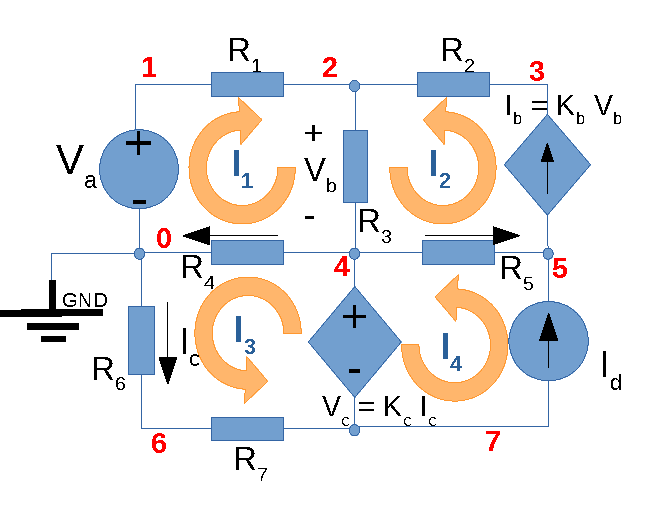
\includegraphics[width=0.6\linewidth]{mesh_diagram.pdf}
\caption{Circuit analyzed in the lab.}
\label{fig:rc}
\end{figure}


To determine the values of the current that goes through the branches of circuit in the Figure~\ref{fig:rc} by the Mesh method, there's only the need to use 4 equations by applying Kirchhoff's voltage law or other relations to obtain the values of 4 unknown values of the currents $I_1$, $I_2$, $I_3$ and $I_4$, as the current of each branch can be obtained by a linear combination of these currents.
	The first equation can be writen as:

\begin{equation}
  I_d = I_4.
  \label{eq:kvl}
\end{equation}

Applying Kirxhhoff's Voltage Law (KVL) to the Mesh with $I_3$ and to the Mesh with $I_1$, we get the following second and third equations:
\begin{equation}
  0 = R_4I_1 + (R_4 + R_6 + R_7-K_c)I3,
\end{equation}

and
\begin{equation}
  V_a(t) = (R_1 + R_3 + R_4)I_1 + R_4I_3 R_3I_2.
  \label{eq:kvl2}
\end{equation}

Knowing that:

\begin{equation}
  I_2 = I_b,
  \label{eq:vo_sol}
\end{equation}

And
\begin{equation}
  v_b = \frac{I_b}{V_b} = \frac{I_2}{V_b}
  \label{eq:vo_nat}
\end{equation}

We get the fourth equation:

\begin{equation}
  I_1(R_3K_b) + I_2(R_3K_b -1) = 0 
\end{equation}

\begin{table}[h]
  \centering
  \begin{tabular}{|l|r|}
    \hline    
    {\bf Name} & {\bf Value [A]} \\ \hline
    @I1[i] & 0.240224 \\ \hline 
@I2[i] & -0.251168 \\ \hline 
@I3[i] & 0.968913 \\ \hline 
@I4[i] & 1.038991 \\ \hline 
@G1[i] & -0.251168 \\ \hline 
@Id[current] & 1.038991 \\ \hline 
@R1[i] & 0.240224 \\ \hline 
@R2[i] & -0.251168 \\ \hline 
@R3[i] & -0.010944 \\ \hline 
@R4[i] & 1.209137 \\ \hline 
@R5[i] & -1.290158 \\ \hline 
@R6[i] & 0.968913 \\ \hline 
@R7[i] & 0.968913 \\ \hline
  \end{tabular}
  \caption{Operating point. A variable preceded by @ is of type {\em current}
    and expressed in Ampere}
  \label{tab:op}
\end{table}

\section{Nodal Method}\label{sec:frequency-response}

In the nodal method, the circuit requires 6 equations to determine the values of V2, V3, V4, V5, V6, V7, which are obtained by applying Kirchhoff's current Law and a relation between the potential difference of two nodes and two other nodes, whose potential difference is imposed by a dependent voltage source. 

Since we considered $V_0$ to be the ground, which means that $V_o$ = 0 and therefore:
\begin{equation}
	V_1 = V_a.
	\label{eq:kvl}
\end{equation}

We get the following equations by applying Kirchhoff's current law at different nodes:

For node 2 we have:
\begin{equation}
	 V_a\frac{1}{R_1} = V_2(\frac{1}{R_1} + \frac{1}{R_2} + \frac{1}{R_3}) + V_3\frac{-1}{R_2} + V_4\frac{-1}{R_3}.
\end{equation}

Node 3:
\begin{equation}
	0 = V_2(\frac{-1}{R_2} - K_b) + V_3\frac{1}{R_2} + V_4(K_b).
\end{equation}

Node 5:
\begin{equation}
	I_d = V_2(K_b) + V_4(\frac{-1}{R_5} - K_b) + V_5\frac{1}{R_5}.
\end{equation}

Node 6:
\begin{equation}
	0 = V_6(\frac{1}{R_6} + \frac{1}{R_7}) + V_7\frac{-1}{R_7} .
\end{equation}

Node 7:
\begin{equation}
	0 = V_4 + V_6(\frac{K_c}{R_6}) - V_7 .
\end{equation}

And finally for node 4:
\begin{equation}
	-I_d = V_2\frac{-1}{R_3} + V_4(\frac{1}{R_3} + \frac{1}{R_4} + \frac{1}{R_5}) + V_5\frac{-1}{R_5} + V_6\frac{-1}{R_7} + V_7\frac{1}{R_7}.
\end{equation}

\begin{table}[h]
  \centering
  \begin{tabular}{|l|r|}
    \hline    
    {\bf Name} & {\bf Value [V]} \\ \hline
    V(1) & 5.239365 \\  \hline 
V(2) & 4.988788 \\  \hline 
V(3) & 4.482071 \\  \hline 
V(4) & 5.023118 \\  \hline 
V(5) & 8.995714 \\  \hline 
V(6) & -1.962948 \\  \hline 
V(7) & -2.972813 \\  \hline 
V(8) & -1.962948 \\  \hline
  \end{tabular}
  \caption{Operating point. The variables are of type {\it voltage} and expressed in
    Volt.}
  \label{tab:op}
\end{table}

